% Chapter 1

\chapter{Starcraft II Machine Learning API} % Main chapter title

\label{chap_api} % For referencing the chapter elsewhere, use \ref{Chapter1} 


%----------------------------------------------------------------------------------------

\section{Environment}
The PySC2 Environment used in this thesis is a python layer on top of the Starcraft II C++ API.
Both of these APIs are relatively new and are still constantly being developed, with new features and actions being added as they evolve. Also, at least the PySC2 API, is still getting big overall changes, that sometimes can even break existing programs relying on an older interface.
PySC2 has been developed specifically for the exploration of reinforcement learning algorithms by a Team of DeepMind developers in collaboration with Blizzard.

\begin{figure}[htb]
  \centering
      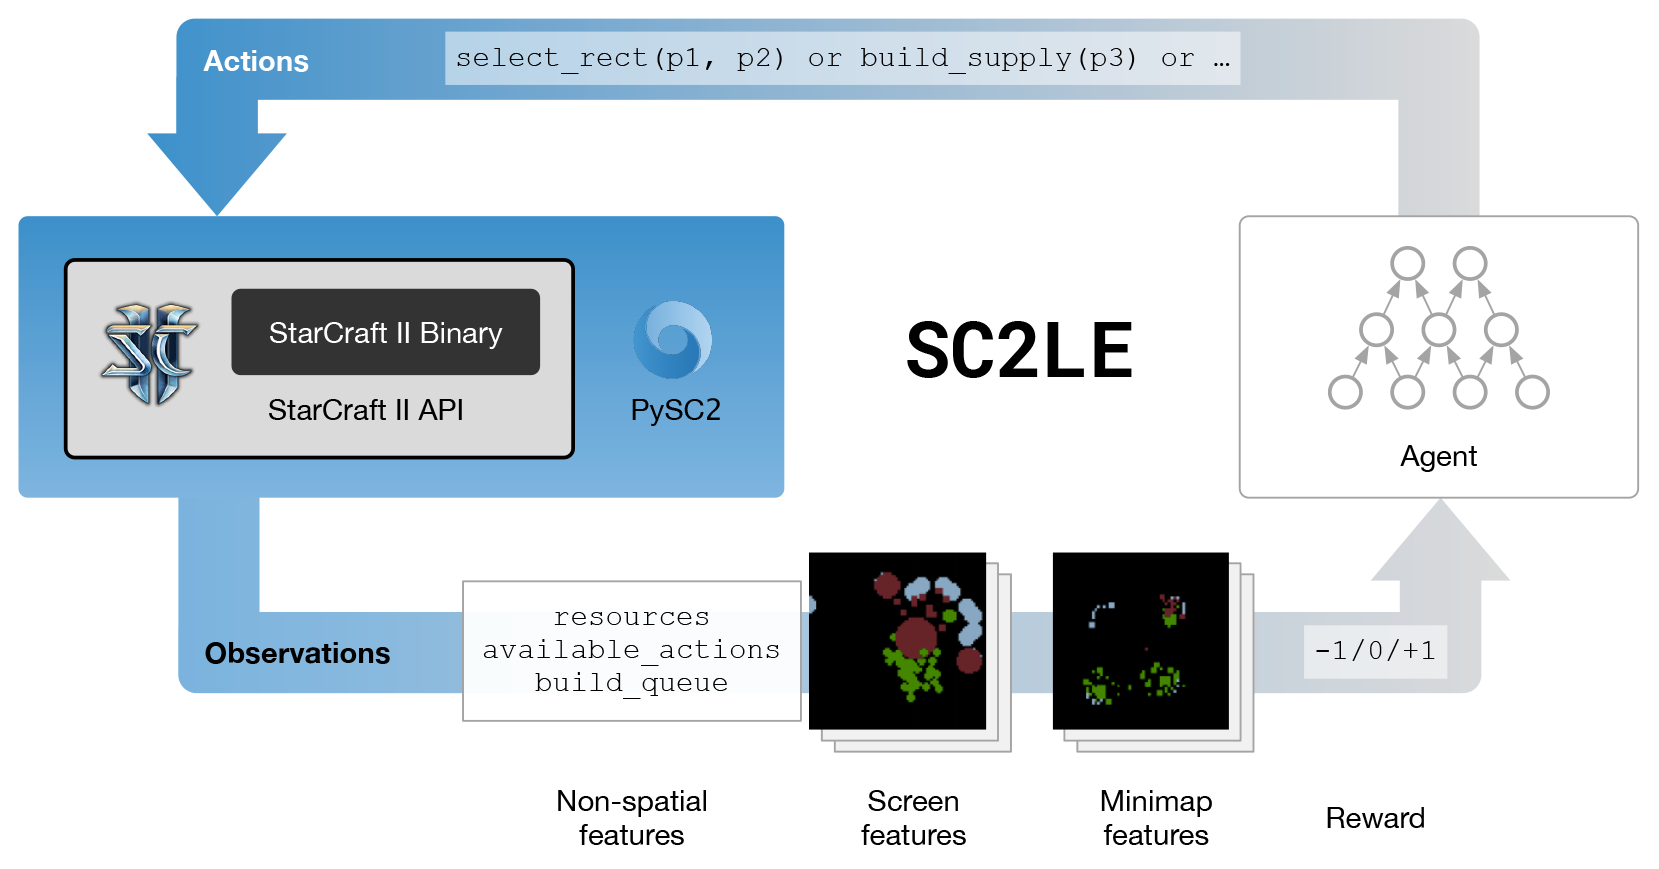
\includegraphics[width=1\textwidth]{Figures/sc2le/sc2le_overview.png}
  \caption{An overview over how an agent interacts with the PySC2 environment. The environment delivers observations in the form of spatial(screen, minimap) information and discrete information. The agent then takes an action in the environment and the cycle continues\citep{DBLP:journals/corr/dmsc2} }
  \label{fig:pysc2_overview}
\end{figure}

Figure \ref{fig:pysc2_overview} shows how the communication between PySC2 and an agent works. PySC2 functions as a wrapper to the StarCraft II machine learning API, which in turn is a wrapper on top of the actual StarCraft II game engine. For each iterative step of an episode the agent can acquire observations for the current state from PySC2 in the form of different types of features. The agent then chooses PySC2 actions on the basis of these observations, which are then executed by PySC2 leading to a new state and thus new observations. This cycle continues until an episode is over.    



\begin{figure}[htb]
  \centering
      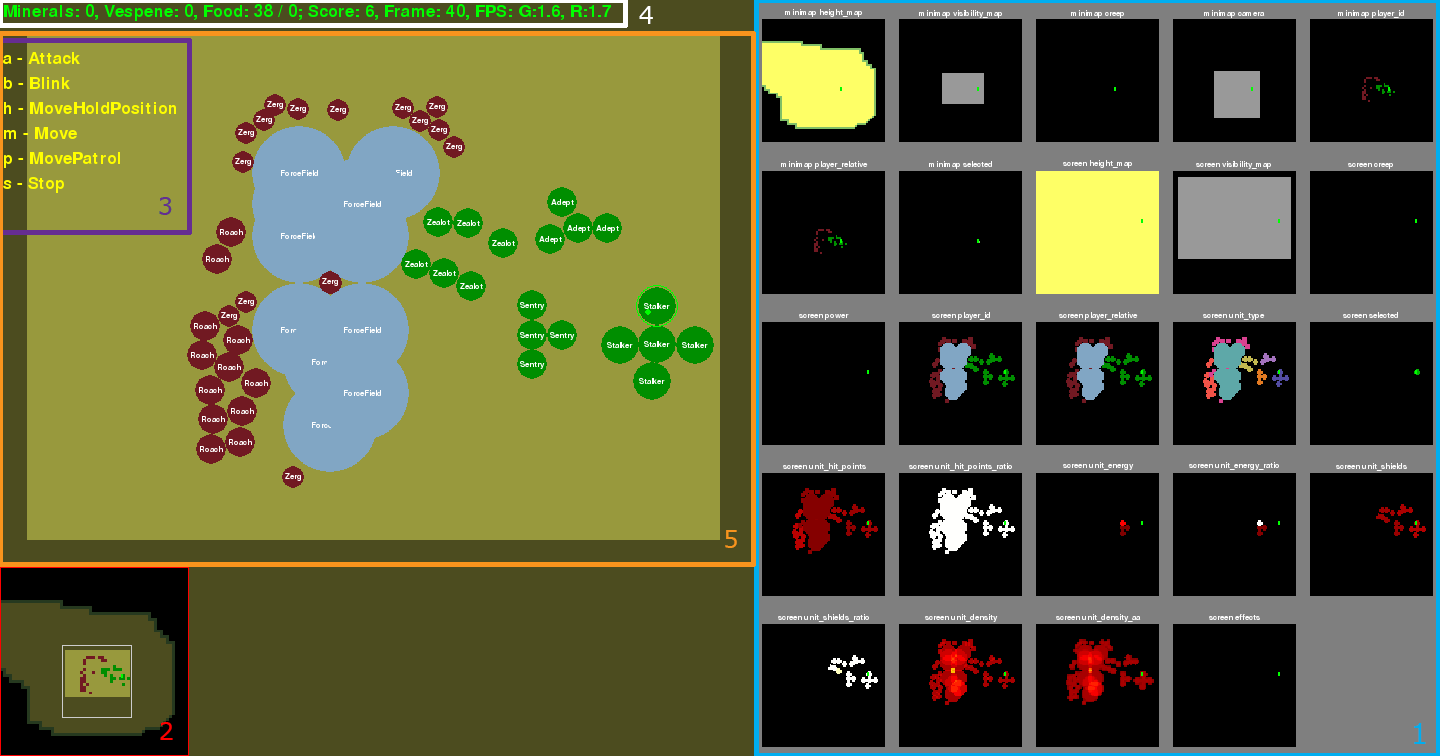
\includegraphics[width=1\textwidth]{Figures/pysc2_borders.png}
  \caption{PySC2 rendered debugging view: 1 - current state of feature layers, 2 - Minimap rendering, 3 - List of available commands, 4 - List of some of the discrete values, 5 - Approximate Game State Render}
  \label{fig:pysc2_render}
\end{figure}
Figure \ref{fig:pysc2_render} shows the debugging view that is provided by the pysc2 framework. This view is particularly important for users of the headless linux client, as the headless client does not offer rendering on it's own as opposed to the Windows and Mac clients.

The right half of this view contains image representations of all feature layers available within PySC2. Section \ref{sec:pysc2_features} discusses those features in greater detail. Altough some of the feature layers in this debug view seem to be multi-colored, this is done only for easier human interpretation. The actual feature layers are all single channel images. Bordered in orange and red are pysc2's depictions of a simplified game view and minimap respectively. On the left side in purple is a list of hotkey - action pairs, that are currently available to player 1. These actions are not stictly StarCraft II actions but specifically PySC2 actions. The top row of information bordered in white is a list of discrete values that PySC2 offers.


\newpage
\subsection{Framework/Engine Parameters}
\label{sec:engparam}
In addition to the specifics of the scenarios created in the Map Editor there are a few parameters for the PySC2 Framework and StarCraft II client, that shape the overall reinforcement learning environment.
Some of the most important are listed here. 

\begin{itemize}  
\item map name - The name of the Map that will be run.
\item screen resolution and minimap resolution - The resolution at which the screen and minimap input layers are rendered by the PySC2 framework.
\item render - A Boolean whether to show a debug view (cf. Figure \ref{fig:pysc2_render}), showing all feature layers and a game view.
\item step multiplier - How many game steps should be taken for every agent step. 
\item score index - Which type of scoring to use. -1 denotes a simple Win/Loss score on a per episode basis. Values >= 0 denote scoring categories within the game with 0 being the cummulative Score.
\item difficulty - the level of AI the agent will play against. 
\item save\_replay - whether StarCraft II should save a .sc2replay file, that can be played back later (can only save roughly 2 million game steps)
\end{itemize}

The screen and minimap resolutions and the step multiplier are particularly important for the performance of reinforcement learning algorithms.
The step multiplier gives control over how often the agent is allowed to act. The game logic itself is calculated at 24 frames per second, meaning that an agent can take a maximum of 24 actions per second. Yet, for most applications this is much too fine-grained and results in too long episodes. The default value of eight game steps per agent has the agent take three actions per second. This is equivalent to a decent to good human player. Of course, if the goal is to beat professional players in complex scenarios increasing this value is unavoidable.

The rendering of the input layers is a very CPU intensive task and a major contributor to the slow performance of the PySC2 environment, which is why setting appropriate screen and minimap resolutions is important. Ideally they should be set as low as possible, while still accurately portraying the game world. The default value of 84 pixels for the screen resolution was used in this project.



\subsection{Features}
\label{sec:pysc2_features}
There are two ways in which PySC2 deals with observations/features. Most of the important features are organized in layers,
and layers in turn are organized in minimap layers and screen layers. Each layer is a very coarsely rendered image map of one specific type of information. The screen layers contain information for the currently active screen of the player, and the minimap layers contain information for the entire map. Using similar resolutions for both map types, which is the default, therefore results in very inaccurate minimap layers that can often miss information. This represents the actual game when it is played by a human though, as the minimap only takes up a very small area on the screen and is only supposed to contain very rough and general information.

As stated in a previous section, the number of layers is still increasing, but at the time of writing there are layers for most of the important types of low level information in the game already available. These include unit type, unit health/shields, unit player affiliation, player visibility, terrain elevation and more.
The second group of features are a set of discrete values, that are not related to screen or minimap coordinates and therefore dont lend themselves well for usage in an image map. Available as discrete values are for example the current resources(minerals, gas, and food) of the player, the current score and saved unit group hotkeys.
The feature layers used specifically in the project for this thesis are

\begin{itemize}
\item player\_relative - Used by all scenarios, it contains pixels with one of five values: 0(No unit), 1(Friendly unit), 2(allied Unit), 3(neutral unit), 4(Enemy unit)
\item creep - values of 0 or 1 depending on whether the terrain is coated with creep or not
\item selected - Values of 0 or 1 depending on whether a unit on the pixel is currently selected by player 1
\item height\_map - values of 0 to ~180 according to terrain elevation, 0 being flat ground
\item unit\_type - values of 0(No Unit) to ~400, representing the id specifying the type of unit on a pixel
\item unit\_hit\_points and unit\_hit\_points\_ratio - How much current health a unit on a pixel has left. The layer unit\_hit\_points contains absolute hit point values, whereas unit\_hit\_points\_ratio contains percentage values normalized to a 0 to 255 range
\item unit\_energy and unit\_energy\_ratio - How much ability energy a unit on a pixel has currently left. As with the hit points layers unit\_energy contains absolute values and unit\_energy\_ratio contains percentages
\end{itemize}
As can be seen, most of these layers have different value ranges and are not normalized to a desired 0 to 255 spectrum that would lend itself well for CNN's. While for some layers like the "creep" and "selected" layers the normalization is trivial, other layers like unit\_type can not easily be normalized, as they contain more than 256 values and floating point values should be avoided.


\subsection{Actions}
Actions in the PySC2 environment work somewhat differently than could be expected in a reinforcement learning environment. Instead of simply having an array of actions, all actions in PySC2 require a number of additional arguments. Most notably many actions need screen coordinates, or information on whether the actions is supposed to be executed directly, or put into an action queue in order to be executed later. 

The actions available in PySC2 are very low level and close to the actions that a human would take, with some simplifications. For example, most actions executed by humans need both a keyboard shortcut(or click on ability symbol) and a mouse click on screen, while PySC2 combines these actions into one. This helps considerably with the limited APM a reinforcement learning algorithm can employ and makes a great deal of sense, as each of these components on their own do not make a successful action.

\begin{figure}[htb]
  \centering
      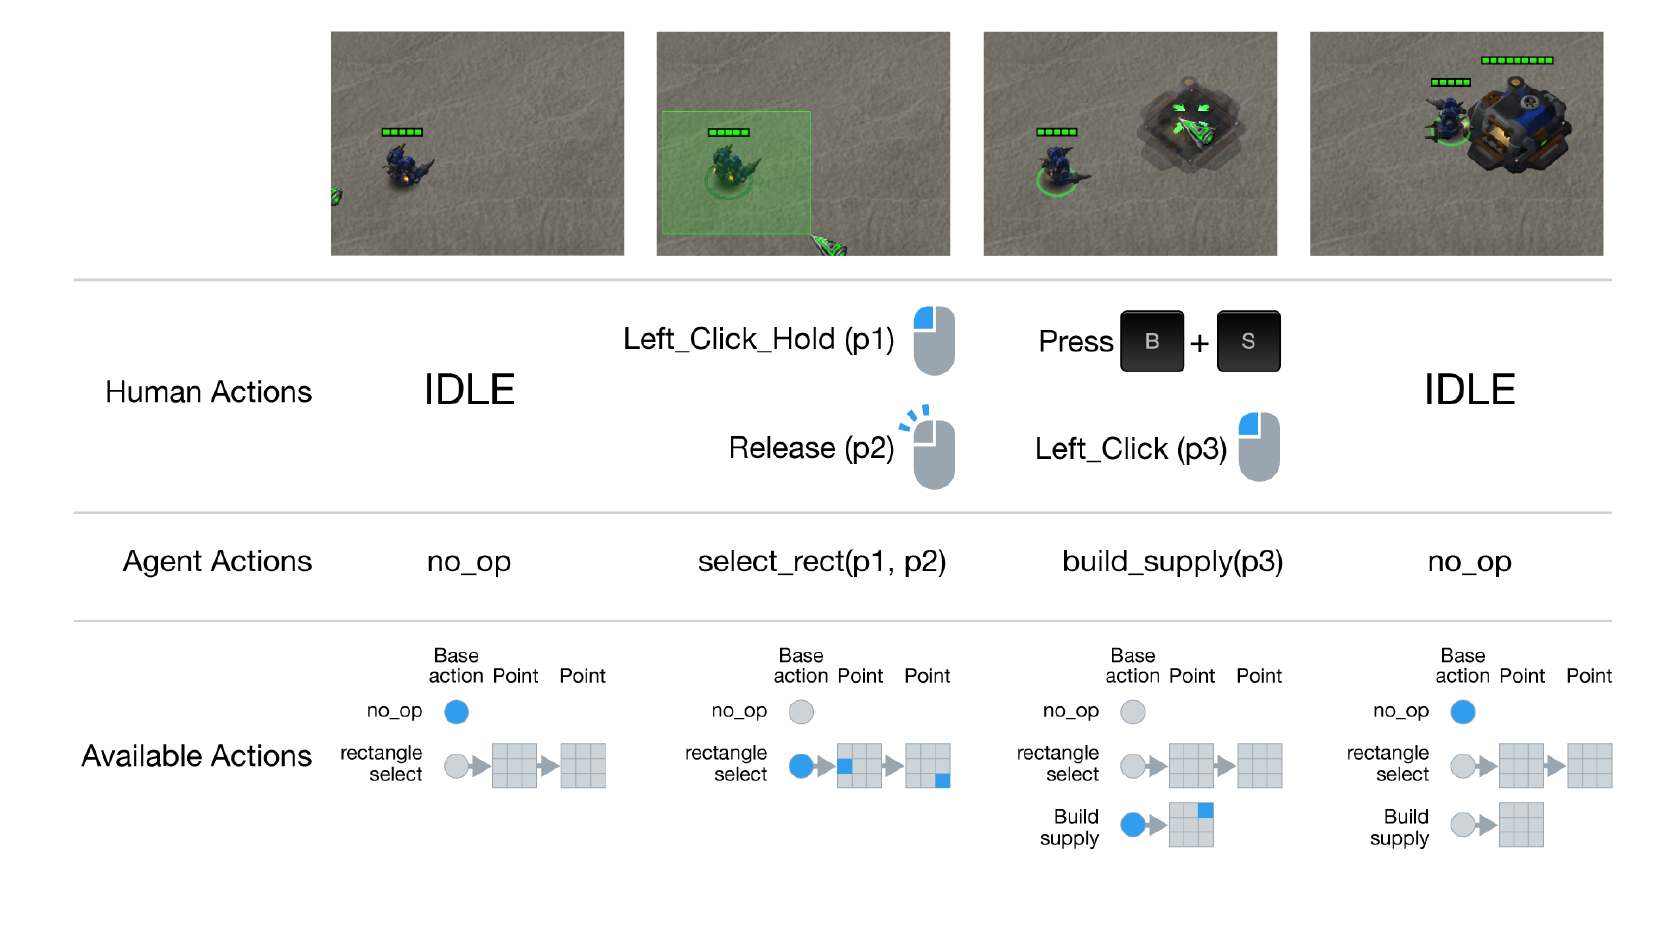
\includegraphics[width=1\textwidth]{Figures/sc2le/sc2le_actions.png}
  \caption{From left to right: a progression of actions and comparison between human actions and the corresponding pysc2 actions \citep{DBLP:journals/corr/dmsc2} }
  \label{fig:pysc2_actions}
\end{figure}
Figure \ref{fig:pysc2_actions} illustrates a sequence of actions a unit could take and how they relate to PySC2 actions. The sequence starts with an idle state, after which the human selects the unit using a rectangle selection and then orders it to build a supply depot. For the actual order to build the supply one can see that even 3 human actions have been combined into a single PySC2 action.


A list of all available actions and their respective arguments can be viewed by executing
\begin{lstlisting}[language=Python]
python -m pysc2.bin.valid_actions
\end{lstlisting}
after installing pysc2. Not all of these actions are available at all times however, as many of these actions depend on having a specific unit or building currently selected.
The actions utilized in the scenarios for this thesis are:
\begin{itemize}
\item No\_op - Have the agent execute no action at all, needs no additional arguments. This is useful in case the current state is preferable over all states that can be achieved by taking an actual action.  
\item Select\_Army - Selects all units belonging to the player on the entire map
\item Move\_Screen - Orders all selected units to move to the specified screen coordinate, without attacking enemy units until the location is reached
\item Attack\_Screen - Similar to Move\_Screen, but ordered units will attack all enemy units they encounter until reaching their destination
\newpage
\item Select\_Point - Selects the unit present at the specified screen coordinate, deselecting all previously selected units. If a friendly unit is selected, it can also be added to the current selection of units instead through the use of the 'shift' modifier in game, or an additional argument in PySc2. In contrast to the real game, enemy units can not be selected at all in PySC2 however. Selecting the background, and in PySC2's case selecting enemy units results in deselecting everything.
\item Effect\_ForceField\_Screen - Orders one of the selected sentry units with enough energy left, to spawn a forcefield at the specified screen coordinate. Will fail if no sentry unit has enough energy. If no sentries are in range of the specified point, one of them will automatically move closer and spawn a forcefield once in range.
\item Effect\_Blink\_Screen - Orders all selected Stalker units to Blink to the specified screen location. Similar to the Force Field ability of the sentry all Stalkers move close enough to the point in order to execute the Blink ability. 
\item Guardian\_Shield\_Quick - Orders one of the selected sentries with enough energy to erect a shield around itself and nearby friendly units by executing the Guardian Shield ability
\end{itemize}

One of the most important actions for human players, \lstinline{select_rect} has been intentionally left out in this project. This is due to the fact, that it is the only available action that not only uses one set of coordinates as parameters, but needs two, one for the upper left and one for the lower right point of the rectangle. This necessitates a different neural network model and increases complexity by a considerable amount(At a resolution of 84 the \lstinline{select_rect} action alone would make for an action space of $84^4$ ). This rectangle selection is commonly used in order to select groups of units. The Rl algorithm instead relies solely on the \lstinline{select_point} method.



\section{Classic Starcraft vs Starcraft II}
In addition to the Starcraft II API there is also a machine learning API for the classic Starcraft: Broodwar.
As both of these games are very similar in their gameplay elements this section illustrates some of the differences of their respective APIs and conclude with why the Starcraft II API was chosen for this thesis.

In contrast to the Starcraft II API input layers, the Starcraft: Broodwar API exposes the features of the environment in an object oriented way. This means, that all players, units, etc. are available as nested objects with discrete values. If, for example, one wants to get all the units of a player one would only have to call getUnits() on the player object and get a list of unit objects with discrete values for position, health, etc.. So while CNNs are almost required for writing bots using the Starcraft II API they are not very useful in the Starcraft: Broodwar API. Not only the features are seperated and bound to these objects though, the actions have to be called on the objects themselves aswell. Hence, ordering a unit to attack would involve simply calling the attack() method on the unit object. 

While this structure of features and actions might seem simpler, it is very unorthodox when considering standard reinforcement learning algorithms and techniques. The Starcraft: Broodwar seems to have been written as a general API for developing Bots with many different technologies and not specifically with reinforcement learning in mind. 

The biggest advantage, that the Starcraft: Broodwar API has to offer for the use in my thesis is that it has been in developement for a much longer time of approximately 3 Years. Accordingly, a community has formed around this API with numerous academic papers being written and examples and tutorials for bots readily available. There are even regular tournaments for StarCraft: Broodwar bots in which teams, mostly universities, let their bots battle against each other. The most notable example is the SSCAIT, which is both a tournament and a ladder \citep{sscait}.

This is opposed to the StarCraft II API, which is very new and therefore has not yet developed such a community.
Also, the StarCraft: Broodwar API offers a full documentation whereas with the StarCraft II a lot of time has to be spend directly looking into the code of the API.

These advantages where however not enough to convince me to use the StarCraft: Broodwar API.
In the end the StarCraft II API was chosen, and specifically PySC2, because it is state of the art, actively being developed, and because it is specifically designed for the use in with reinforcement learning algorithms.


